\documentclass[12pt, letterpaper]{article}
\usepackage{graphicx}
\usepackage{caption}
\usepackage[hidelinks]{hyperref}
\graphicspath{{images/}}

\begin{document}
    \begin{titlepage}
    \begin{center}
        \vspace*{1cm}
            
        \Huge
        \textbf{Project Modeling Report}
            
        \vspace{0.5cm}
        \LARGE
        Thermal Scanning App
            
        \vspace{1.5cm}
            
        \textbf{Colter Roche, Jose Bastardo}
            
        \vfill
          
        \Large
        Senior Design 1\\
        COP4934C.01\\
        \today
            
    \end{center}
\end{titlepage}
    \newpage
    \tableofcontents
    \newpage
    \listoffigures
    \newpage
    \section{Project Background}
    \paragraph{}
    Corserva is a managed IT service provider that develops and sells custom software and hardware solutions. Corserva's customers
    include hospitality and other in-person focused related businesses. Official CDC guidelines to businesses encourage taking steps to 
    prevent the spread of Covid-19 among employees and customers, including temperature checks. Corserva has sponsored this project 
    to produce a thermal screening solution capable of processing people quickly and without requiring user interaction to minimize additional
    contact.
    \paragraph{}
    Preliminary development and testing has already been completed by Corserva. The system uses a thermal and a regular 
    camera to recognize users and read the temperature of their face. If the temperature is above a certain threshold, 
    then an alert is shown and the flagged person can be moved aside for further screening.  The first iteration of the thermal app has several problems:
    \begin{itemize}
        \item The camera suffers from temperature drift over time and required frequent callibration.
        \item The facial recognition process is around 5 seconds, limiting the rate people can be processed.
        \item Onboarding new users requires interaction directly through the app, not practical for large numbers of employees.
        \item No option to send an alert to the scanned user.
    \end{itemize}
    The new application developed as part of this project will address these problems.
    \section{Scope}
    \subsection{Project Scope}
    \paragraph{}
    The scope of this project is to produce an application and companion mobile application 
    to measure and report high temperatures of people passing through the system. The 
    thermal camera will use an auto calibration system to increase accuracy of 
    readings. Mobile application to smooth the onboarding process and provide reports 
    to users.
    \subsection{Business Scope}
    \paragraph{}
    The business scope is to provide business with a kiosk and mobile app system that will make 
    it easier for them to maintain safety precautions during the current Covid 19 
    pandemic while also increasing the speed in which staff and customers can enter their place of business.
    \section{System Overview}
    \subsection{Users}
    Those who will benefit and be affected by the new solution include:
    \begin{itemize}
        \item Attendant - The new app will no longer require frequent calibration, lessening the need for supervision and technical troubleshooting.
        \item Corserva - The app will be well structured and extensible, allowing for relative ease when adding new features.
        \item Customers - The streamlined onboarding system for users will alleviate concerns to do with overcrowding and long wait times to register in person. 
        \item End Users - Users will receive a notification and report in the companion app after they are scanned, increasing their health awareness.
    \end{itemize}
    \subsection{Location}
    \paragraph{}
    The system can be installed anywhere with electrical power and space for a callibration object. The companion app
    will be available for Android and IOS.
    \subsection{Responsibilities}
    \paragraph{}
    The primary responsibilities of the new system are:
    \begin{itemize}
        \item Accurately measure the temperature of people passing through the scanner
        \item Automatically recalibrate the thermal camera to account for possible drift
        \item Report people with a facial temperature higher than 100 degrees to the attendant
        \item Recognize users based on facial imaging, and send an alert to them via the companion app
        \item Provide real-time reporting of scans and locations to the customer
        \item Provide report history to users through companion app
        \item Register new users including facial recognition models through companion app 
    \end{itemize}
    Other desired features include:
    \begin{itemize}
        \item Process multiple people passing through the system at a time
        \item Cross-platform support for the thermal scanning app
    \end{itemize}
    The system will not be responsible for medical screenings or temperature verification.
    \newpage
    \section{User Requirements}
    \subsection{Interfaces}
    \paragraph{}
    The thermal scanner system will need to interface with the chosen facial recognition system and the companion app. 
    Corserva included code for facial recognition from another project as one possible solution.
    \subsection{Outputs}
    \paragraph{}
    The thermal app will display a UI alert to the operator if a user has a high temperature.  The app also sends personal reports
    to the user's companion app when a new scan is performed, and updates a general database for larger reports.
    \subsection{Inputs}
    \paragraph{}
    The mobile app will ask the user for their first name, last name, email, password, and 
    it will user their camera to take photos extract facial recognition data. 
    The app will then send that information to the database. The thermal app will use 
    the thermal camera to scan a user at the kiosk to gather facial recognition data 
    and their temperature.  The customer is able to configure settings for their deployment through the thermal scanner app UI.
    \subsection{Processing}
    \paragraph{}
    Not applicable to this project. The thermal scanner system is not intended for medical use beyond preliminary
    screenings. 
    \subsection{Data Storage}
    \paragraph{}
    All the necessary data will be stored in a database cloud using a MariaDB 
    Relational Database Service from Amazon Web Services. The database will contain 
    users first and last name, email and password, facial recognition data, and a 
    record of past temperature scans.
    \newpage
    \section{Functional Decomposition Diagrams}
    \begin{figure}[h!]
        \centering
        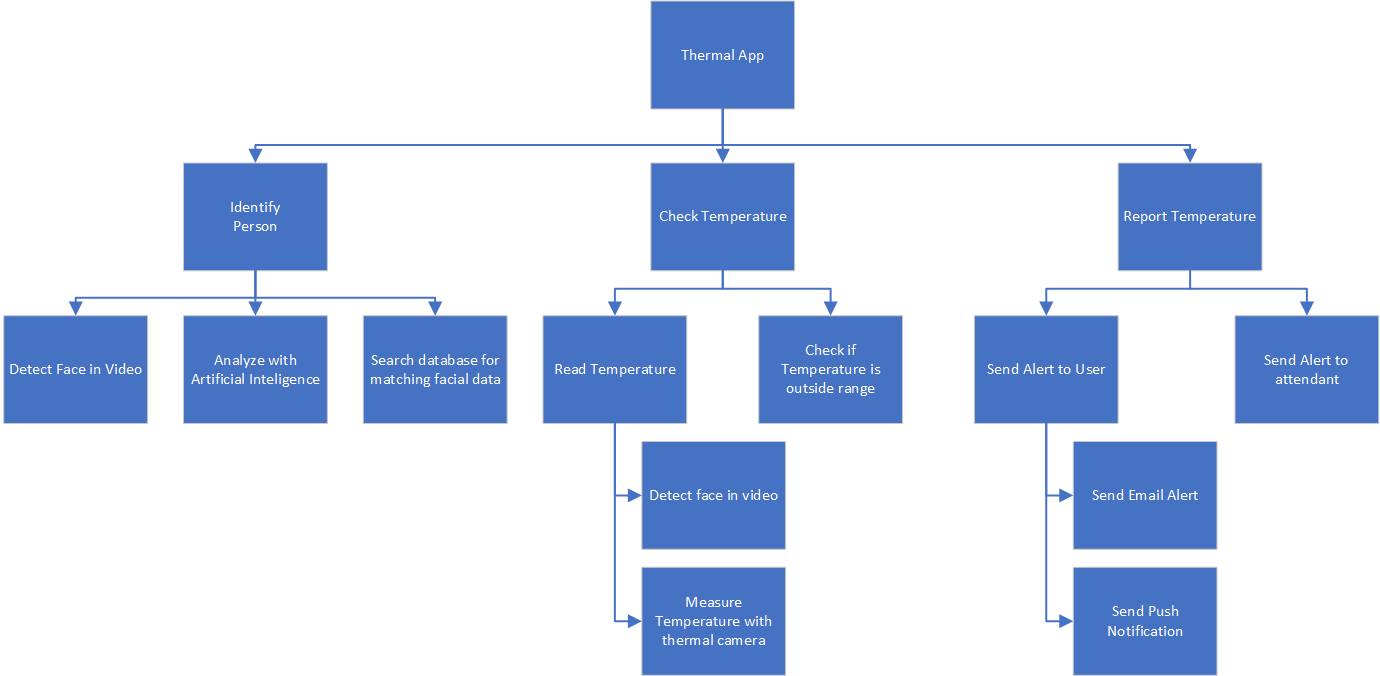
\includegraphics[width=0.8\textwidth]{Function diagram-Thermal App.png}
        \caption{Functional Decomposition Diagram - Thermal scanner}
    \end{figure}
    \begin{figure}[h!]
        \centering
        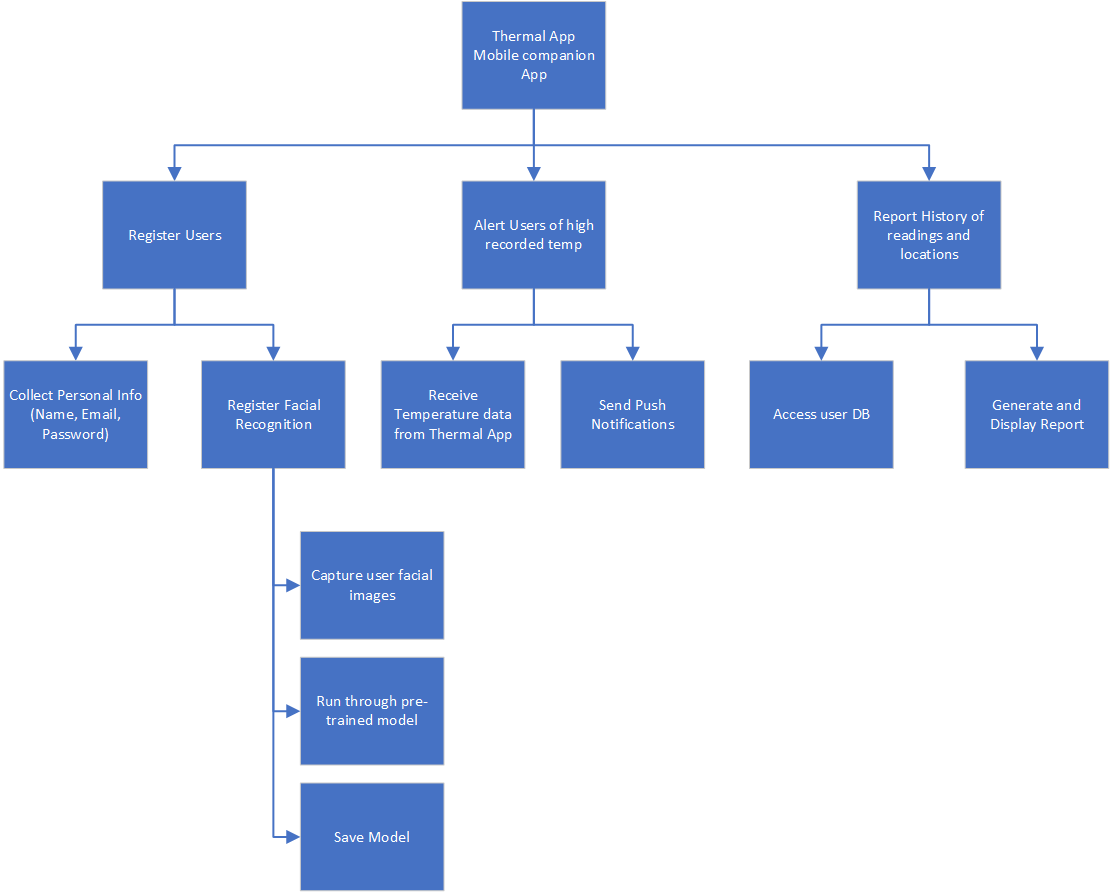
\includegraphics[width=0.8\textwidth]{Function diagram-Mobile Comapanion App.png}
        \caption{Functional Decomposition Diagram - Comapanion App}
    \end{figure}
    \newpage
    \section{Data Flow and Application Structure}
    \begin{figure}[h!]
        \centering
        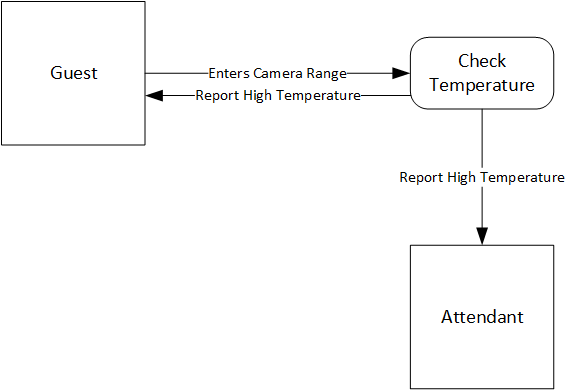
\includegraphics[width=0.8\textwidth]{DFD Top Level.png}
        \caption{Top Level Data Flow Diagram}
    \end{figure}
    \begin{figure}[h!]
        \centering
        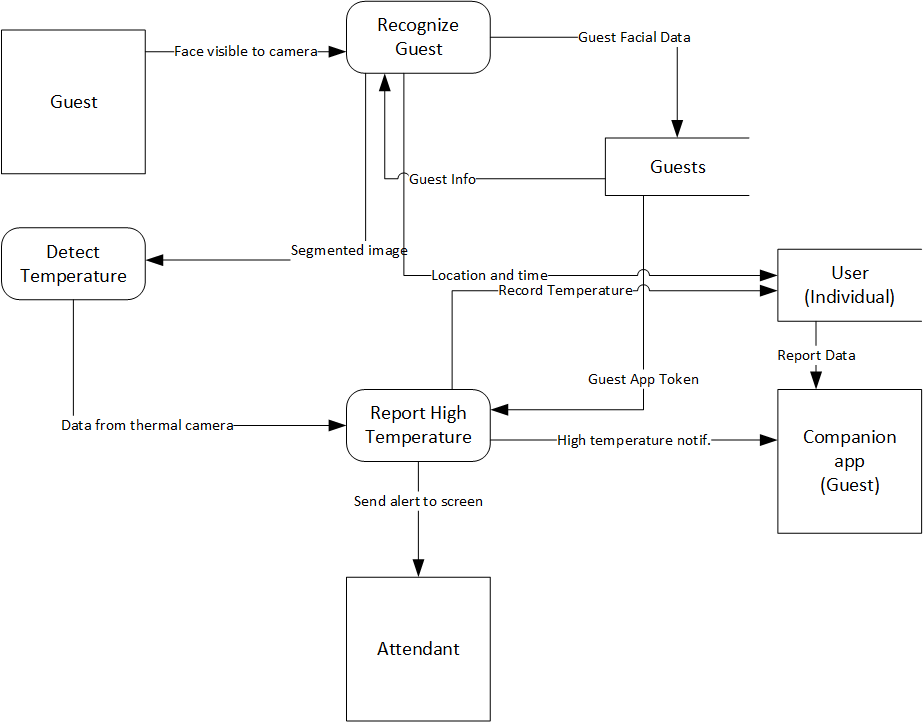
\includegraphics[width=0.8\textwidth]{DFD Level 1.png}
        \caption{Level 1 Data Flow Diagram}
    \end{figure}
    \begin{figure}[h!]
        \centering
        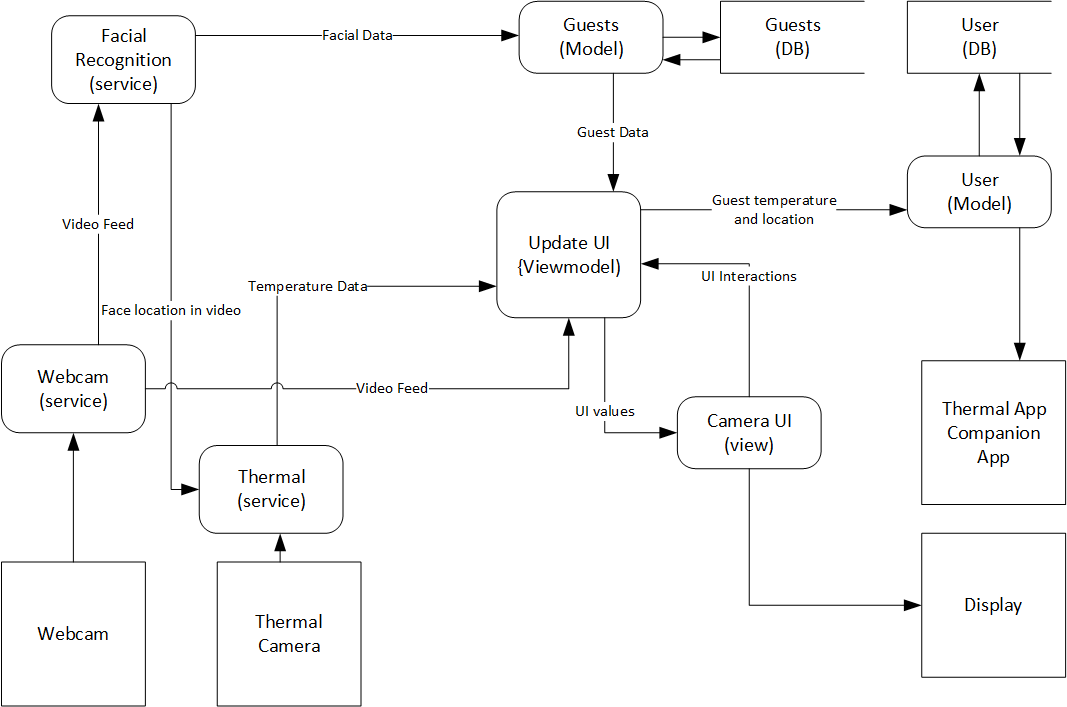
\includegraphics[width=0.8\textwidth]{DFD Level 2.png}
        \caption{Level 2 Data Flow Diagram}
    \end{figure}
    \newpage
    \section{Gantt Chart}
    \begin{figure}[h!]
        \centering
        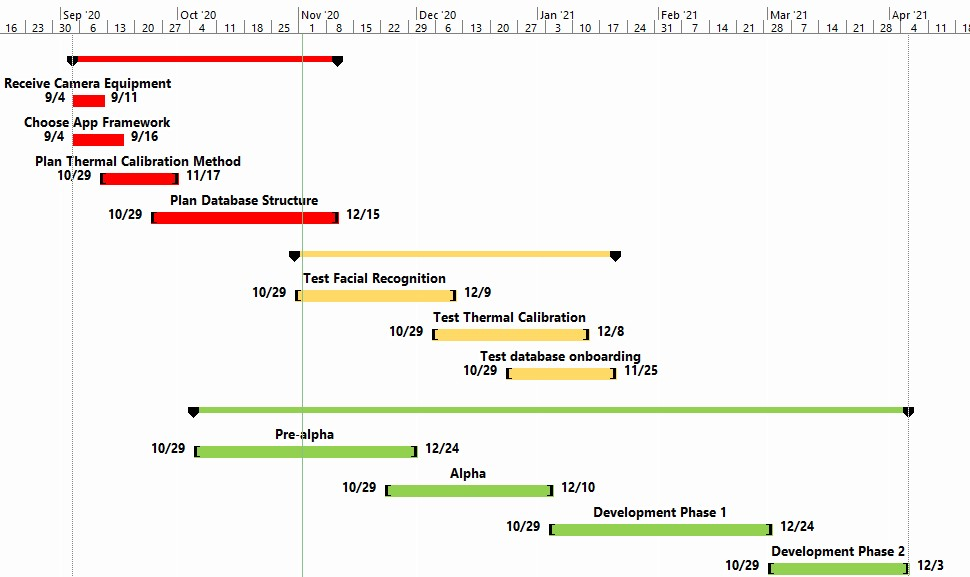
\includegraphics[width=0.8\textwidth]{Gantt Chart v3.jpg}
        \caption{Gantt Chart for Thermal App Development}
    \end{figure}
    \section{Team Member Participation}
    Participation was split as follows:
    \begin{itemize}
        \item Colter Roche: 60\%
        \item Jose Bastardo: 40\%
    \end{itemize}
\end{document}